\documentclass[12pt,letterpaper]{report}

\usepackage{booktabs}
\usepackage{csvsimple}
\usepackage{pgfplotstable}
\usepackage{pgfplots}
\pgfplotsset{compat=1.16}
%\usepackage[letterpaper,top=1in,bottom=1in,right=1in,left=1in]{geometry}
\usepackage{multirow}
\usepackage{caption}
\usepackage{fancyhdr}
\usepackage{textcomp}
\usepackage{siunitx}

\pagestyle{fancy}
\lhead{Modeling Documentation}
\chead{Do Not Copy}
\rhead{Cypress Confidential}
\lfoot{}
\cfoot{Page \thepage}
\rfoot{}

\begin{document}

\section{Introduction}
\subsection{Revision History}


\section{My Graph}
In this section I've included a graph. It's cold in here. Not as cold as last week.
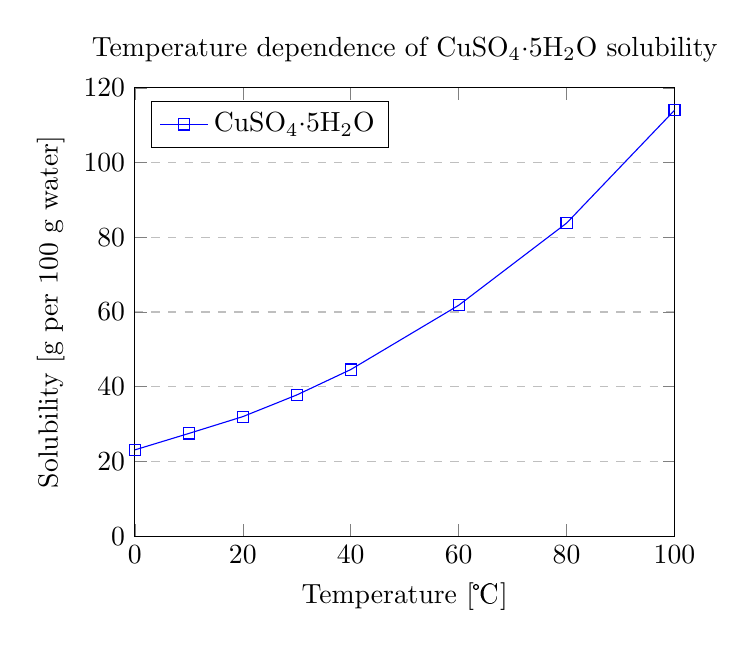
\begin{tikzpicture}
\begin{axis}[
    title={Temperature dependence of CuSO$_4\cdot$5H$_2$O solubility},
    xlabel={Temperature [\textcelsius]},
    ylabel={Solubility [g per 100 g water]},
    xmin=0, xmax=100,
    ymin=0, ymax=120,
    xtick={0,20,40,60,80,100},
    ytick={0,20,40,60,80,100,120},
    legend pos=north west,
    ymajorgrids=true,
    grid style=dashed,
]
 
\addplot[
    color=blue,
    mark=square,
    ]
    coordinates {
    (0,23.1)(10,27.5)(20,32)(30,37.8)(40,44.6)(60,61.8)(80,83.8)(100,114)
    };
    \legend{CuSO$_4\cdot$5H$_2$O}
 
\end{axis}
\end{tikzpicture}

\section{My First Table}
\begin{center}
\captionof{table}{This is my table}
\begin{tabular}{@{}llr@{}} \toprule
\multicolumn{2}{c}{Item} \\ \cmidrule(r){1-2}
Animal & Description & Price (\$)\\ \midrule
Gnat & per gram & 13.65 \\
     & each     & 0.01 \\
Gnu  & stuffed  & 92.50 \\
Emu  & stuffed  & 33.33 \\
Armadillo & frozen & 8.99 \\ \bottomrule
\end{tabular}
\end{center}

\section{My Table}
In this section I've included a table. The quick brown fox jumps over the lazy dog.
\begin{center}
\captionof{table}{This is my table}
\begin{tabular}{ |c|c|c|c| } 
\hline
Version & Date & Author & Memo \\
\hline
1.0 & 2018/01/04 & RCWA & Hello World \\
\hline
1.1 & 2018/01/15 & RCWA & First update\\
\hline
2.0 & 2018/02/12 & RCWA & Version 2.0 \\ 
\hline
\multirow{2}{*}{2.1} & \multirow{2}{*}{2018/03/30} & \multirow{2}{*}{RCWA} & Lots of updates:\\ 
 & & & Like this one \\
\hline
\end{tabular}
\end{center}

\captionof{table}{This is my table}
\csvautotabular{simple.csv}
\centering

\end{document}
